\section{Sistema de equações lineares – concentração de reatores}

Sistema de equações são vistos com frequência em problemas que envolvem a engenharia química. Com o princípio de conservação das massas, vários problemas são modelados utilizando essas entidades matemáticas. Talvez o exemplo mais famoso é o que envolve vários reatores ligados entre si. O princípio de conservação de massas resulta em balanços efetuados em um “recipiente” (no caso um reator) expressos matematicamente por:

\begin{center}
	Acumulação = Entrada – Saídas
\end{center}

\begin{figure}[H]
	\centering
	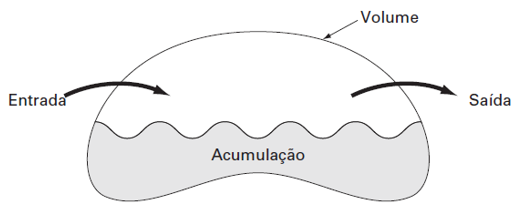
\includegraphics[width=0.8\textwidth]{./Imagens/Sistema de eq/sis1.png}
	\caption{Conservação da massa}
	\label{fig:sis1}
\end{figure}

Caso as entradas sejam maiores que saídas, têm – se um aumento da massa no interior, caso contrário, as saídas sejam maiores que as entradas, a massa no interior diminui. Chamamos de estado estacionário, ou regime permanente, quando o somatório das entradas se iguala ao somatório das saídas. Dessa forma o acúmulo é zerado e sobra:

\begin{center}
Entrada = Saídas
\end{center}

Imagine a seguinte situação. 5 reatores em série conectados entre sim, nos quais a alimentação de um ou mais reatores é a saída de um ou mais reatores, como mostra a imagem a seguir:

\begin{figure}[H]
	\centering
	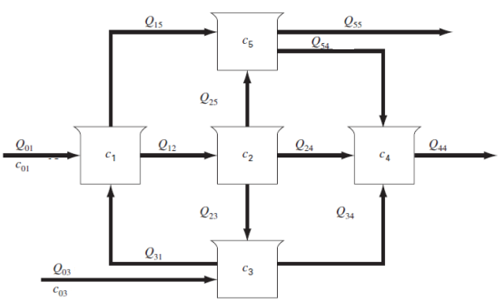
\includegraphics[width=0.8\textwidth]{./Imagens/Sistema de eq/sis2.png}
	\caption{Esquema de reatores}
	\label{fig:sis2}
\end{figure}

Na qual $Q_{ij}$ (vazão) representa a saída do reator $i$ alimentando o reator $j$. Por exemplo, $Q_{24}$ informa que uma das saídas do reator 2 alimenta o reator 4. As concentrações de cada reator são denotadas pelos $c_{i}$ ($i = 1, 2, ..., 5$). A taxa de massa que sai (ou entra) em cada reator é calculada multiplicando a vazão, dada em  $\large \frac{m^3}{min}$ , com a concentração dada em $\large \frac{mg}{m^3}$. 

Para o reator 1, há duas entradas e duas saídas como indicam as setas na figura acima, então o balanço de massa fica:

\begin{equation}
\large Q_{01} c_{01}  + Q_{31} c_{3}  = Q_{15} c_{1}+ Q_{12} c_{1}
\tag{13.1}
\end{equation}

Vamos aplicar método numérico para resolver situação – problema semelhante da figura acima, onde os valores das vazões são fornecidos, como as concentrações que alimentam os reatores 1 e 3. O objetivo é determinar as concentrações dos 5 reatores ($c1, c2, c3, c4, c5$). 
As razões fornecidas são: 

$$
\large Q_{01} = 5, Q_{31} = 3, Q_{25} = 2, Q_{23} = 2
$$

$$
\large Q_{15} = 4, Q_{55} = 3, Q_{54} = 3, Q_{34} = 7
$$

$$
\large Q_{12} = 4, Q_{03} = 8, Q_{24} = 0, Q_{44} = 10, c_{01} = 10, c_{03} = 20
$$

Repetindo o procedimento acima, para os 5 reatores, temos o seguinte sistema:

$$\large 8c_{1}  - 3c_{3}  = 50$$

$$\large 4c_{1}  - 4c_{2}  = 0$$

$$\large 10c_{3}  - 2c_{2}  = 160$$

$$\large -7c_{3} + 10c_{4} - 3c_{5}  = 0$$

$$\large 4c_{1}  +2c_{2}  -6c_{5}  = 0$$

O sistema acima pode ser reescrito na forma de multiplicação matricial, do tipo:

\begin{equation}
\large Ax + b = 0
\tag{13.2}
\end{equation}

Onde $A$, no nosso caso, representa a matriz 5x5 dos coeficientes do sistema
acima, $x$ é o vetor coluna 5x1 com os valores das concentrações que queremos determinar, por último, $b$ é vetor coluna dos componentes independentes.

$$\large A = \begin{bmatrix} 8 & 0 & -3 & 0 & 0 \\ 4 & -4 & 0 & 0 & 0 \\ 0 & -2 & 10 & 0 & 0 \\ 0 & 0 & -7 & 10 & -3 \\ 4 & 2 & 0 & 0 & -6 \end{bmatrix}$$

$$\large b = \begin{bmatrix} -50 \\ 0 \\ -160 \\ 0 \\ 0 \end{bmatrix}$$

$$\large x = \begin{bmatrix} C_{1} \\ C_{2} \\ C_{3} \\ C_{4} \\ C_{5} \end{bmatrix}$$

Utilizando o \textbf{Linsolve}, função embutida para o Scilab, podemos resolver o sistema acima e encontrar os valores das concentrações. A função linsolve calcula todas as soluções para problemas do tipo $\large Ax + b = 0$.

\begin{minted}{Scilab}
// sistema de equações algébricas lineares
// utilizaremos a função Linsolve para 
// resolver um sistema simulando a 5 reatores ligados entre si
// Queremos determinar as concetrações 
// c1, c2, c3, c4, c5 (referente a cada reator)

clear, clc

//informe aqui a seu sistema do tipo Ax + b = 0
A = [8 0 -3 0 0;4 -4 0 0 0;0 -2 10 0 0; 0 0 -7 10 -3;4 2 0 0 -6] 
// matriz dos coeficientes
b = [-50; 0; -160; 0; 0] 
x = linsolve(A, b)

printf("O vetor x é: \n")
mprintf("C1 = %6.4f \n", x(1))
mprintf("C2 = %6.4f \n", x(2))
mprintf("C3 = %6.4f \n", x(3))
mprintf("C4 = %6.4f \n", x(4))
mprintf("C5 = %6.4f \n", x(5))
\end{minted}